\documentclass[11pt]{article}
\usepackage[letterpaper,margin=1in,centering]{geometry}
\usepackage{graphicx}
\usepackage{subfigure}
\usepackage{amssymb}  
\usepackage{amsmath}
\usepackage{amsfonts}
\usepackage{siunitx}
\usepackage{mathtools}
\usepackage{microtype}
\usepackage{color}
\usepackage{bm}
\usepackage{xr-hyper}
\usepackage{hyperref}
\usepackage[]{cleveref} % get fancy referencing

\externaldocument[]{manuscript}[manuscript.pdf]

% edit cref citations for IEEE format
\crefformat{equation}{(#2#1#3)} % no abbreviation for equation numbers
\Crefformat{equation}{Equation~(#2#1#3)} % no abbreviation for equation numbers
\crefrangeformat{equation}{(#3#1#4--#5#2#6)}
\Crefrangeformat{equation}{(#3#1#4--#5#2#6)}
\crefmultiformat{equation}{(#2#1#3)}{ and~(#2#1#3)}{, (#2#1#3)}{ and~(#2#1#3)}
% edit cref citations for IEEE format
\crefformat{figure}{Fig.~#2#1#3} % no abbreviation for equation numbers
\Crefformat{figure}{Fig.~#2#1#3} % no abbreviation for equation numbers
\crefrangeformat{figure}{Figs.~#3#1#4--#5#2#6}
\Crefrangeformat{figure}{Figs.~#3#1#4--#5#2#6}
\crefmultiformat{figure}{Figs.~#2#1#3}{ and~#2#1#3}{, #2#1#3}{ and~#2#1#3}
% for items in a list
\crefformat{enumi}{(#2#1#3)}
\Crefformat{enumi}{Item~(#2#1#3)} 
\crefrangeformat{enumi}{(#3#1#4--#5#2#6)}
\Crefrangeformat{enumi}{Items~(#3#1#4--#5#2#6)}
\crefmultiformat{enumi}{(#2#1#3)}{ and~(#2#1#3)}{, (#2#1#3)}{ and~(#2#1#3)}



%%%%%%%%%%%%%%%%%%%%%%%%%
% CUSTOM MACROS
%%%%%%%%%%%%%%%%%%%%%%%%%
\newcommand{\linearize}[3]{\ensuremath{\left. \frac{\partial #1}{\partial #2} \right|_{#3} \delta #2}}
\newcommand{\norm}[1]{\ensuremath{\left\| #1 \right\|}}
\newcommand{\Real}[1]{\ensuremath{\Re \left\{ #1 \right\}}}
\newcommand{\bracket}[1]{\ensuremath{\left[ #1 \right]}}
\newcommand{\braces}[1]{\ensuremath{\left\{ #1 \right\}}}
\newcommand{\parenth}[1]{\ensuremath{\left( #1 \right)}}
\newcommand{\pair}[1]{\ensuremath{\langle #1 \rangle}}
\newcommand{\met}[1]{\ensuremath{\langle\langle #1 \rangle\rangle}}
\newcommand{\refeqn}[1]{(\ref{eqn:#1})}
\newcommand{\reffig}[1]{Fig. \ref{fig:#1}}
\newcommand{\tr}[1]{\mathrm{tr}\ensuremath{\negthickspace\bracket{#1}}}
\newcommand{\trs}[1]{\mathrm{tr}\ensuremath{[#1]}}
\newcommand{\deriv}[2]{\ensuremath{\frac{\partial #1}{\partial #2}}}
\newcommand{\diff}[2]{\ensuremath{\frac{d #1}{d #2}}}
\newcommand{\dirDiff}[2]{\ensuremath{\mathbf{D}_{#2} #1 \cdot \delta #2}} % directional derivative
\newcommand{\SO}{\ensuremath{\mathsf{SO(3)}}}
\newcommand{\T}{\ensuremath{\mathsf{T}}}
\renewcommand{\L}{\ensuremath{\mathsf{L}}}
\newcommand{\so}{\ensuremath{\mathfrak{so}(3)}}
\newcommand{\SE}{\ensuremath{\mathsf{SE(3)}}}
\newcommand{\se}{\ensuremath{\mathfrak{se}(3)}}
\newcommand{\R}{\ensuremath{\mathbb{R}}}
\newcommand{\aSE}[2]{\ensuremath{\begin{bmatrix}#1&#2\\0&1\end{bmatrix}}}
\newcommand{\ase}[2]{\ensuremath{\begin{bmatrix}#1&#2\\0&0\end{bmatrix}}}
\newcommand{\D}{\ensuremath{\mathbf{D}}}
\newcommand{\Sph}{\ensuremath{\mathsf{S}}}
\renewcommand{\S}{\Sph}
\newcommand{\J}{\ensuremath{\mathbf{J}}}
\newcommand{\Ad}{\ensuremath{\mathrm{Ad}}}
\newcommand{\intp}{\ensuremath{\mathbf{i}}}
\newcommand{\extd}{\ensuremath{\mathbf{d}}}
\newcommand{\hor}{\ensuremath{\mathrm{hor}}}
\newcommand{\ver}{\ensuremath{\mathrm{ver}}}
\newcommand{\dyn}{\ensuremath{\mathrm{dyn}}}
\newcommand{\geo}{\ensuremath{\mathrm{geo}}}
\newcommand{\Q}{\ensuremath{\mathsf{Q}}}
\newcommand{\G}{\ensuremath{\mathsf{G}}}
\newcommand{\g}{\ensuremath{\mathfrak{g}}}
\newcommand{\Hess}{\ensuremath{\mathrm{Hess}}}
\newcommand{\refprop}[1]{Proposition \ref{prop:#1}}
\newcommand{\mypaper}{}
\newcommand{\vecbf}[1]{\bm{#1}}
\newcommand{\slfrac}[2]{\left.#1\middle/#2\right.}

\newcommand{\RNum}[1]{\uppercase\expandafter{\romannumeral #1\relax}}
\newcommand{\RI}{\text{\RNum{1}}}
\newcommand{\RII}{\text{\RNum{2}}}
\newcommand{\RIII}{\text{\RNum{3}}}

\newenvironment{correction}{\begin{list}{}{\setlength{\leftmargin}{1cm}\setlength{\rightmargin}{1cm}}\vspace{\parsep}\item[]``}{''\end{list}}

\begin{document}

%\pagestyle{empty}

\section*{Response to the Reviewers' Comments for JCAS-D-16-00607}

I would like to thank the reviewers for their thoughtful comments, which are aimed towards improving the quality of the paper and the clarity of the results. 
In accordance with the comments and suggestions, the paper has been revised, and the answers to all comments are addressed as follows.

(In the revised manuscript, the citation numbers for equations, assumptions, propositions, and references are changed. This answer is written according to the new item numbers.)

\subsection*{Reviewer 2}

\textit{A new geometric adaptive control scheme for the stabilization of the attitude dynamics of a rigid body with state inequality constraints is studied in this paper and ensures that the closed-loop system is asymptotically stable in the sense of Lyapunov stability. The main contribution and result are well presented and organized. Therefore, it is sufficient to be accepted in this journal provided that the following minor problems are considered in the revised version.
}

% \setlength{\leftmargini}{0pt}
\begin{enumerate}

\item \textit{ In general, the external disturbance is a time-varying signal even though it is bounded. Thus, authors should consider the time-varying disturbance case.}

It is true that typically, the external disturbances on a system will be time varying.
However, the form of uncertainty shown in \( (1) \) is commonly used in the adaptive control literature~\cite{lee2013b,ioannou2012}.
As a result, we use this same form of uncertainty, namely that the uncertain disturbance is additive in nature and enters through the input channel.
In addition, a wide variety of disturbances in the aerospace engineering field are accurately represented by this formulation and several examples are given in the article.
Furthermore, it has been shown in~\cite{ioannou2012} that this form of adaptive control is able to handle time-varying uncertainties in which the uncertain term is varying sufficiently slowly as compared to the controlled dynamics. 
We have improved the manuscript with an additional numerical experiment in~\Cref{ssec:time_varying} demonstrating the ability of the adaptive controller to handle time-varying disturbances.
The additional content is duplicated here:
\begin{correction}
    The form of the uncertainty, given in~\cref{eqn:Wdot}, is commonly used in the adaptive control literature~\cite{lee2013b,ioannou2012}. 
    A wide variety of realistic disturbances, such as gravitational gradients or malfunctioning thrusters, are accurately represented via this model. 
    In addition, it is possible to represent the uncertainty of a time-varying inertia matrix as an equivalent external disturbance. 
    For example, Euler's law gives the relationship for the rate of change of angular momentum
    \begin{align*}
        M_{ext} = \dot{\vecbf{H}} = \dot{J} \vecbf{\Omega} + J \dot{\vecbf{\Omega}} .
    \end{align*}
    Using this, we can see that an instantaneous change in \( J \) is proportional to an external moment.
    Finally, it has been shown that this adaptive control formulation is able to handle time-varying disturbances under some mild assumptions~\cite{ioannou2012}. 

    We demonstrate the ability to handle an uncertain time-varying disturbance via numerical example.
    The system is identical to the one presented in~\Cref{sec:numerical_simulation}, however we modify the external disturbance. 
    The external disturbance is the superposition of constant and time-varying terms as
    \begin{align*}
        \Delta = \begin{bmatrix} 0.2 \\ 0.2 \\0.2 \end{bmatrix} + 0.02 \begin{bmatrix} \sin 9 t \\ \cos 9 t \\ \frac{1}{2} \parenth{\sin 9t + \cos 9t}\end{bmatrix} \si{\newton\meter}.
    \end{align*}
    We define a constraint in the inertial frame as \( v = [\frac{1}{\sqrt{2}}, \frac{1}{\sqrt{2}}, 0]^T \) with \( \theta = \ang{12} \).
    The initial state is defined as \(R(0) = \exp( \frac{\pi}{2} \hat{e}_3) \), while the desired state is \(R_d =I \).
    The goal is to rotate the vehicle about the \( e_3 \) axis while avoiding the obstacle and compensating for the time-varying disturbance. 

    \Cref{fig:tv} demonstrates the ability for the adaptive controller, which is presented in Proposition~\ref{prop:adaptive_control}, to handle time-varying disturbances.
    \Cref{fig:Psi_tv} shows the non-dimensional value of the configuration error function and demonstrates that the adaptive controller is able to stabilize the system to the desired attitude configuration.
    In addition,~\cref{fig:con_angle_tv} shows that the constraint is never violated as the angle between the body-fixed sensor \( r \) and the constraint \( v \) is greater than \SI{12}{\degree} over the entire attitude maneuver.
    We can see in~\cref{fig:Delta_tv} that that estimate \(\bar \Delta \) for each of the components, accurately tracks the true disturbance after approximately~\SI{5}{\second}.

    \begin{figure}
        \centering 
        \subfigure[{Configuration error \( \Psi \)}  ]{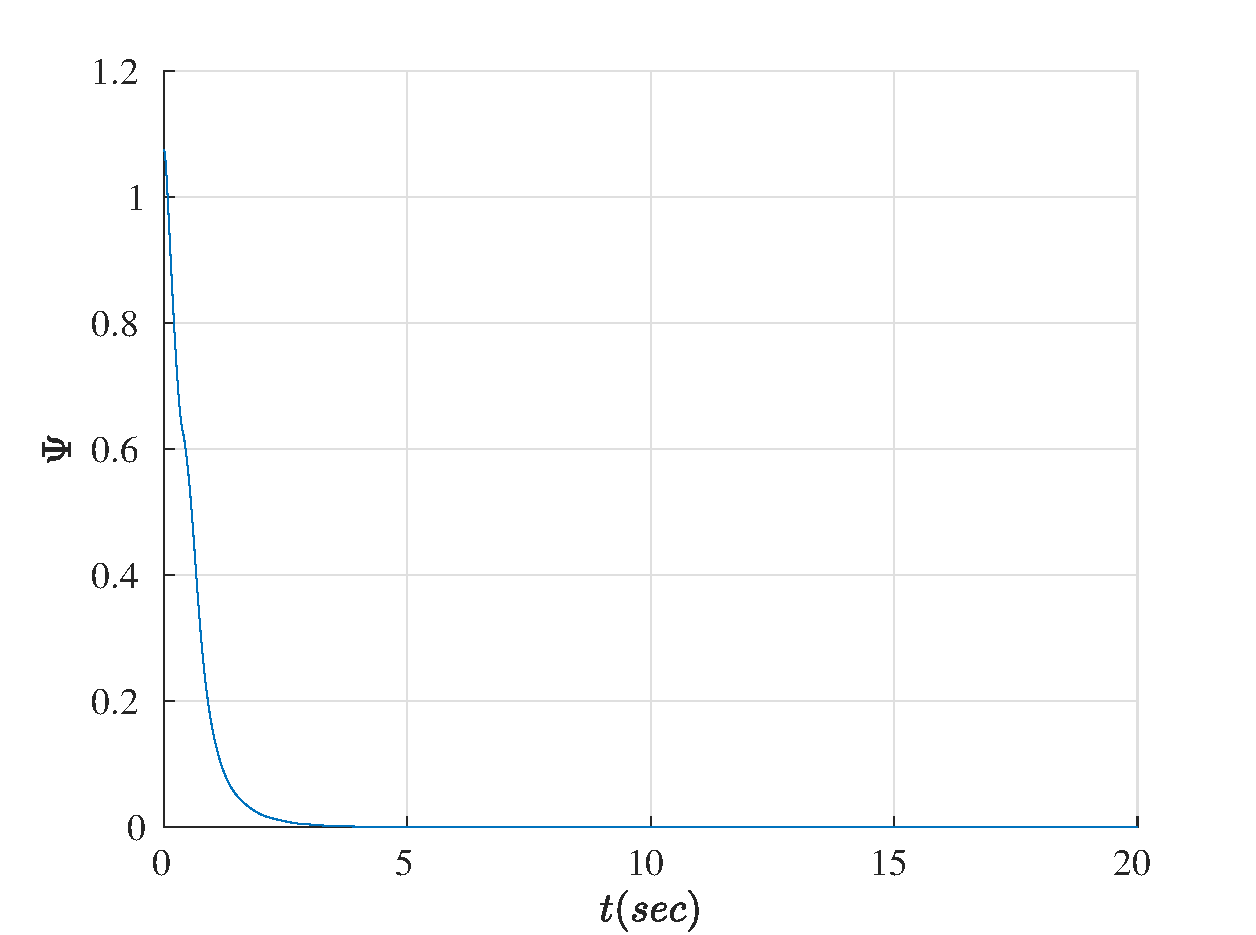
\includegraphics[width=0.3\columnwidth]{figures/Psi_tv} }~
        \subfigure[{Angle to constraint } ]{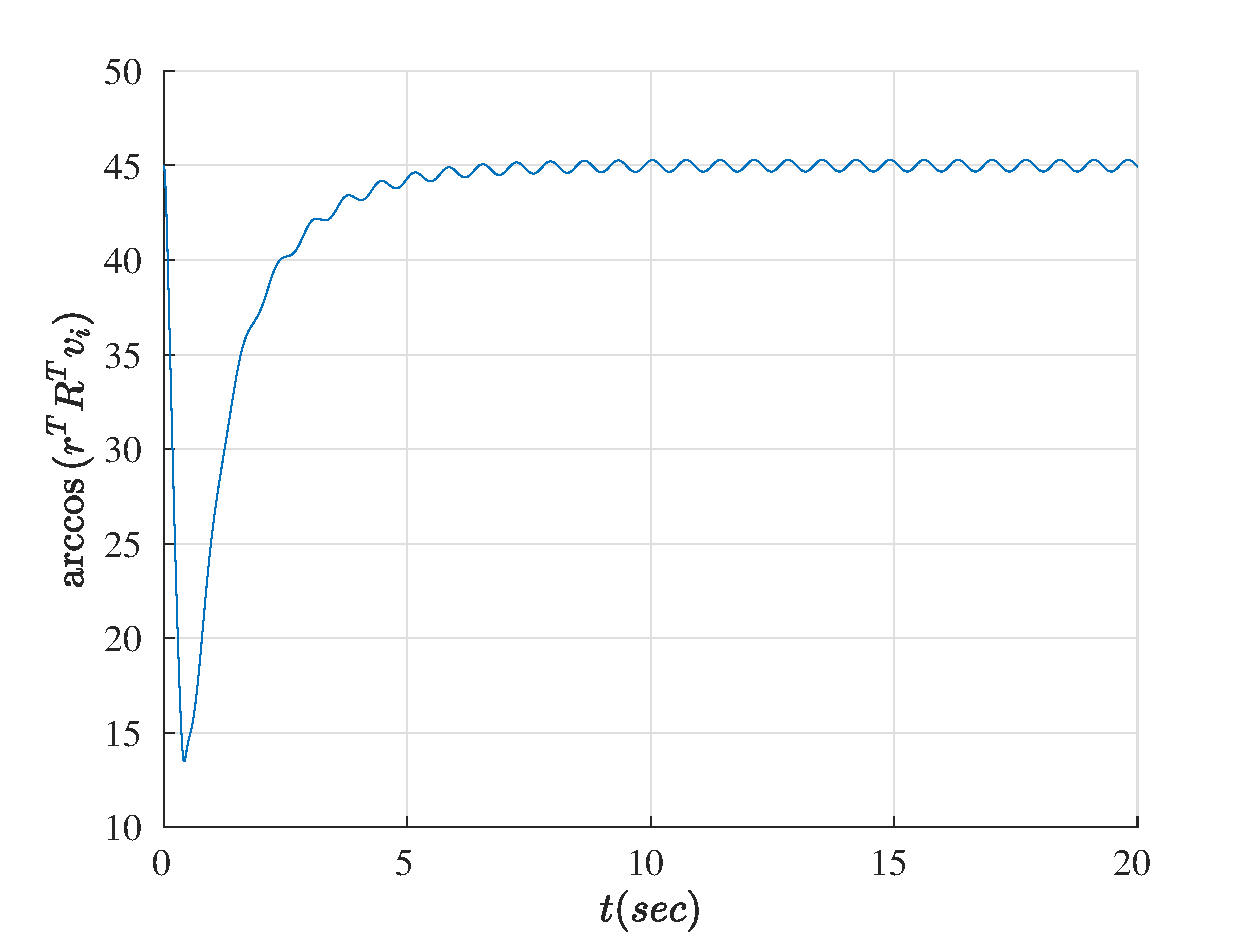
\includegraphics[width=0.3\columnwidth]{figures/constraint_angle_tv.pdf} }~
        \subfigure[{Disturbance estimate \(\bar\Delta\) components} ]{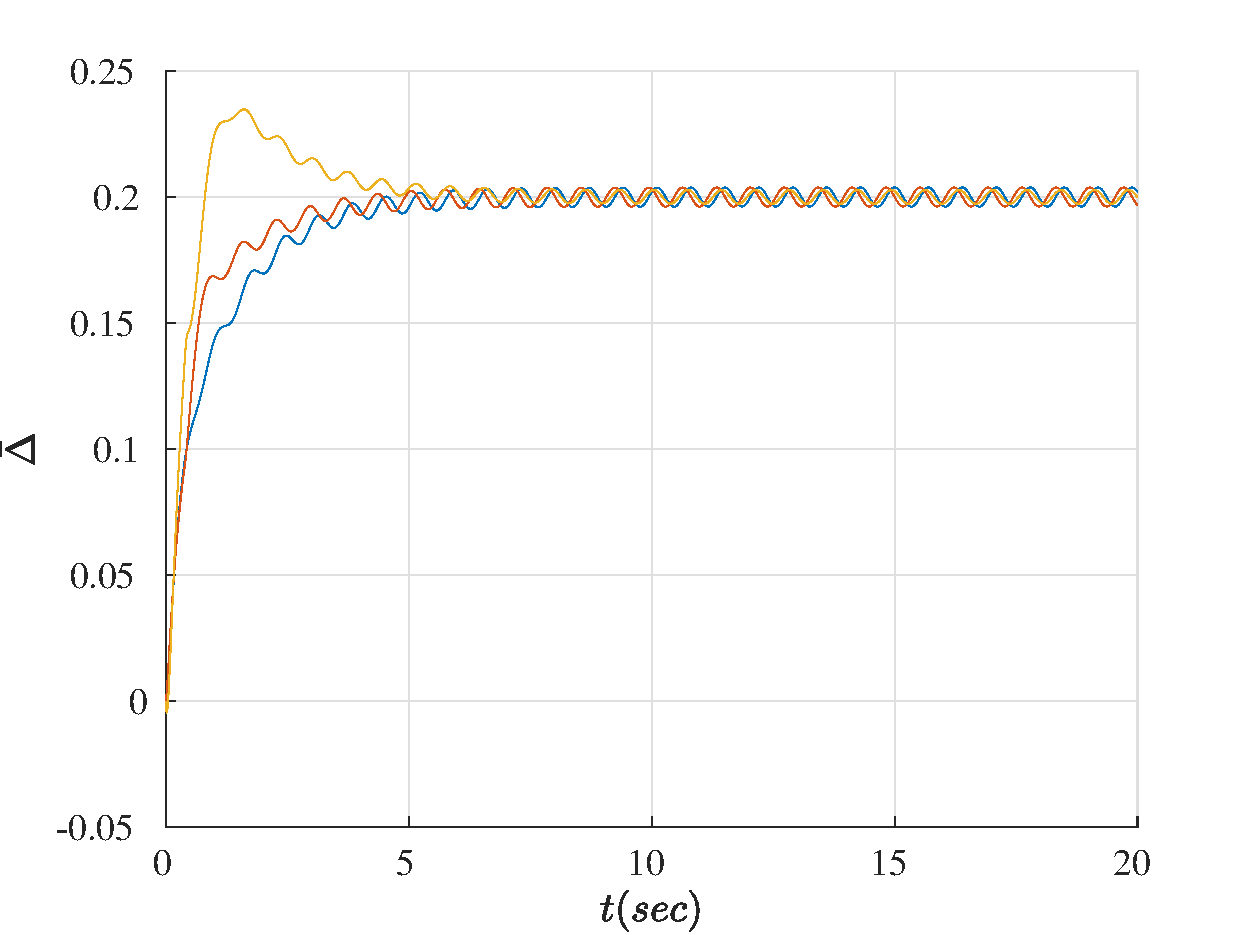
\includegraphics[width=0.3\columnwidth]{figures/delta_tv} }
        \caption{Time-varying external disturbance simulation}
         
    \end{figure}

\end{correction}
\item \textit{If the inertia matrix is unknown, how to modify the suggested control system guaranteeing the asymptotic stability?}

In this work, we are focused on the design of attitude controllers in the presence of state inequality constraints. 
The addition of an adaptive update law allows the system to stabilize in the presence of unknown external disturbances.
We are not considering the case of an unknown inertia matrix, but rather assume that there exists accurate knowledge of the rigid body. 
This assumption is relatively simple to satisfy as any physical control system will first have an accurate model of the system itself.
For example, the mass and inertia properties of all spacecraft are accurately measured and verified prior to launch. 

In addition, the uncertainty model presented in the paper is commonly used in the adaptive control literature.
Also, it is possible to represent a uncertain or varying inertia matrix as an external disturbance torque. 
Additional detail has been added to the manuscript in~\Cref{ssec:time_varying} and is duplicated in the previous answer.

\item \textit{The state inequality constraint is not violated based on adding the repulsive term in the attitude error function. Is this result still valid if this constraint becomes time-dependent?}

In this work, we are specifically concerned with presenting a geometric attitude controller on \( \SO \) in the presence of state inequality constraints.
More specifically, we are assuming that these constraints are time-invariant rather than time dependent. 
This type of constraint is representative of the attitude constraints that are frequently experienced in the attitude control of spacecraft. 
For example, various keep-out zones for sensitive electro-optical sensors are well represented as a fixed constraint in the inertial frame. 
In addition, the time scale of the attitude dynamics, and therefore any attitude control maneuver, is much shorter than the time scale of the translational dynamics.
In other words, a time-dependent constraint in the inertial frame will evolve at a much slower rate as compared to the attitude dynamics. 
As a result, it is possible to model the time-varying constraints as a series of time-invariant constraints in the inertial frame. 
In this situation, the presented approach allows for a straightforward method to design an attitude stabilization control law. 
However, this is a very good suggestion and it is an area of current research effort.

\end{enumerate}

\subsection*{Reviewer 3}

\textit{This paper considers the attitude control with inequality constraints. Attitude dynamics with matched uncertainty which is parameterized by a unknown constant matrix, and hard constants expressed by rotation matrix are considered. Although the problem is very interesting, the proofs for major results on the case with plant uncertainty are far from complete. Some comments are listed below.}

\begin{enumerate}
\item \textit{Please give a precise definition of variation used in the paper, e.g., eq. (17) and (18)}
The variation of the rotation matrix is defined as
\begin{align*}
    \delta R = \left. \diff{}{\epsilon} \right|_{\epsilon=0} R \exp{\epsilon \hat{\eta}} = R \hat{\eta} .
\end{align*}
We have augmented the proof of Proposition 1, which is given in Appendix 1, to include the definition of the variation as:
\begin{correction}
The infinitesimal variation of a rotation matrix is defined as
\begin{align*}
    \delta R = \left. \diff{}{\epsilon} \right|_{\epsilon=0} R \exp{\epsilon \hat{\eta}} = R \hat{\eta} .
\end{align*}
\end{correction}

\item \textit{This is serious. In section 2, the upper bounds listed in Proposition 4 are given. Well, these should be the properties that your controller guarantees not come from the set D you've defined. Since these properties are used to derive the bound H which is used to derive the result in Proposition 5, the stability proof under the proposed controller is far from complete.}

Lyapunov stability is valid if the given properties of \( V \) are satisfied in an open neighborhood of the desired attitude configuration. 
The presented details, which are shown in~\Cref{proof:att_control,proof:eR_dot_bound}, are valid in the selected domain \( D \) about the desired attitude.
Therefore, Lyapunov stability is valid if \( D \) is also an open neighborhood of the desired attitude.

The set \( D = \braces{R \in \SO \vert \Psi < \psi < h_1, r^T R^T v < \beta < \cos \theta} \) of the metric space \( \parenth{R \in \SO, \Psi(R,R_d)} \) is an open neighborhood of \( R_d \) if there exists an \( \epsilon > 0 \) such that for any \( R \in \SO | \Psi(R,R_d) < \epsilon \), it is also true that \( R \in D \).
The selected domain \( D \) excludes the undesired equilibrium points of \( A(R) \) and the infeasible regions defined by the constraints \( r^T R^T v_i \), i.e. the desired attitude should be sufficiently far away from the constraints. 
We can ensure that \( D \) is an open neighborhood of \( R_d \) by choosing \( \epsilon = \min \braces{\psi, \Psi(R|r^T R^T v = \beta,R_d)}\).
Therefore, the given domain \( D \) is an open neighborhood of the desired attitude configuration, \(R_d\), and the Lyapunov stability results are valid in this domain.

The domain \( D \) is chosen to both exclude the undesired critical points of \( A(R)\) as well as the infeasible regions defined by the constraints. 
In general, this is not a difficult assumption to satisfy as the desired attitude will typically be located far from the constrained regions.
We have augmented the manuscript with some additional discussion of the chosen domain \( D \) in~\Cref{proof:eR_dot_bound}.

\begin{correction}
    We choose the domain \( D \) to exclude the undesired critical points of \( A(R) \) as well as the infeasible regions defined by the state inequality constraints. 
    Furthermore, one can show that the set \( D \) is an open neighborhood of the desired attitude configuration, \( R_d\).
    Therefore, the selected domain ensures that the configuration error function is bounded \( \Psi < \psi \).
    This implies that that both \( A(R) \) and \( B(R) \) are bounded by constants \( c_A c_B < \psi < h_1\).
    Furthermore, since \( \norm{B} > 1 \) this ensures that \( c_A, c_B < \psi\) and shows~\cref{eqn:AB_bound}.
\end{correction}

\item \textit{Typo in eq. (40).}

The equation has been modified as:
\begin{correction}
\begin{gather}
    0 < c < \frac{4 k_R k_\Omega}{k_\Omega^2 + 4 k_R \lambda_M H} ,
\end{gather}
\end{correction}

\item \textit{Abuse of notation 'hat' and 'vee' in equations (6)-(8)}

The \( \wedge : \R^3 \to \so \) and \( \vee : \so \to \R^3 \) operators are used according to the convention that is common in the literature~\cite{lee2010,lee2011a}.
In this case, the \textit{hat} operator is equivalently represented as \( \hat{x} = \parenth{x}^\wedge \).
This representation enables a consistent notation for both short/simple terms, such as \( \hat{x} \) and more complicated terms such as \(\parenth{\hat{e}_\Omega R^T R_d G + (R^T R_d G)^T \hat{e}_\Omega}^\vee\). 
Finally, this dual usage of the notation drastically improves the quality of the resulting typography.

\end{enumerate}

\subsection*{Reviewer 4}
\textit{This paper presents a new geometric adaptive control system with state inequality constraints for the attitude dynamics of a rigid body. The controlled attitude trajectory avoids undesired regions defined by the inequality constraint, and an adaptive update law that enables attitude stabilization in the presence of unknown disturbances is developed. However, the paper can be improved and some revisions are required.}

\begin{enumerate}
\item \textit{Probably, the weak point is that the underlying experiments are not solid. The author claims that the attitude dynamics and the proposed control systems are developed on the special orthogonal group such that singularities and ambiguities of other attitude parameterizations, such as Euler angles and quaternions are completely avoided.  But the numerical simulations and experimental results don't demonstrate the effectiveness of the proposed control system. How is the singularity avoided in the Euler angles? Please give the detail.}

The primary purpose of this article is to present the formulation of constrained attitude control on the special orthogonal group, \( \SO \).
There have been many references which have explicitly demonstrated the issues of singularities and ambiguities of other attitude parameterizations~\cite{chaturvedi2011a,bhat2000,hughes2004,shuster1993}.
As a result, the numerical simulations and hardware experiments were designed to demonstrate the feasibility of the proposed attitude control and the application of general attitude constraints on \( \SO \), rather than highlight the deficiencies of attitude parameterizations.
However, additional detail has been added in the numerical simulation section demonstrating and highlighting the singularities inherent in the Euler angle parameterization and is given in~\Cref{ssec:attitude_parameterization}.

\begin{correction}
    Attitude parameterizations, such as Euler angles and Quaternions, are frequently used in the aerospace and astrodynamics communities~\cite{vallado2007}.
For example, Euler angle sequences are frequently used to describe the transformation between a variety of reference frames used to describe the position and orientation of the orbit of Earth satellites~\cite{vallado2007}.
In addition, quaternions were used during the operation of Skylab and the NASA Space Shuttle~\cite{hughes2004}.
However, the choice of attitude parameterization plays a critical role in control design and the resulting motion of the system.

% singularities and the problems involved with using Euler angles
Euler angle sequences are a minimum, three-parameter set of angles which describe the transformation between two reference frames.
Using Euler angles, we can represent any general rotation as a sequence of three intermediate rotations~\cite{shuster1993}.
By convention, there are \num{24} possible Euler angle sequences for any given rotation.
In addition, Euler angles are a minimum representation, as only three angles, and the associated sequence, are required to describe the three angular degrees of freedom of the rigid body.
However, there is great ambiguity in the representation of the attitude as there are many equivalent Euler angle sequences for a given attitude of the system.
Therefore, great care must be taken in the control system design to ensure that a consistent sequence is used. 
Furthermore, it has been shown that no minimal attitude representation can describe orientations both globally and without singularities~\cite{hughes2004,bhat2000}.
These singularities can cause significant difficulties during control design and hardware implementation.

To demonstrate the effect of the kinematic singularities inherent with Euler angles we will represent the attitude of the body fixed reference frame, \( \vecbf{b}_i \), with respect to the inertial frame, \( \vecbf{e}_i\), in terms of the \( 3-1-3\) Euler angle sequence.
More explicitly, this corresponds to the rotation sequence \( \theta_1 \vecbf{b}_3 , \theta_2 \vecbf{b}_1, \theta_3 \vecbf{b}_3 \).
The rotation matrix, \( R(\theta_1, \theta_2, \theta_3) \), corresponding to this sequence is 
\begin{align}\label{eq:euler313}
    \begin{bmatrix}
        -s_1 c_2 s_3 + c_3 c_1 & -s_1 c_2 c_3 - s_3 c_1 & s_1s_2 \\
        c_1 c_2 s_3 + c_3 s_1 & c_1 c_2 c_3 - s_3 s_1 & - c_1 s_2 \\
        s_2 s_3 & s_2 c_3 & c_2
    \end{bmatrix} ,
\end{align}
where \( s_i, c_i \) represent \( \sin \theta_i, \cos \theta_i \) for \( i = \braces{1,2,3}\).
Using this representation that kinematic differential equations for the associated Euler angles are given as
\begin{align}\label{eq:euler313_diff}
    \begin{bmatrix}
        \dot{\theta}_1 \\ \dot{\theta}_2 \\ \dot{\theta}_3 
    \end{bmatrix}
    =
    \begin{bmatrix}
        \slfrac{\parenth{\Omega_1 s_3 + \Omega_2 c_3}}{s_2} \\
        \Omega_1 c_3 - \Omega_2 s_3 \\
        -\slfrac{\parenth{\Omega_1 s_3 + \omega_2 c_3}c_2}{s_2} + \Omega_3
    \end{bmatrix} .
\end{align}
From~\cref{eq:euler313_diff}, it is immediately clear that a singularity exists when \( \sin \theta_2 = 0 \) or equivalently, \( \theta_2 = 0, \pm \pi \). 
In the vicinity of the singularity, the angular velocities of the Euler angles will tend to approach \( \pm \infty \) and the angular velocities will experience instantaneous sign changes.
Furthermore, all Euler angle sequences will exhibit a similar singularity at either \( \theta_2 = 0, \pm \pi \) or \( \theta_2 = \pm \frac{\pi}{2}, \pm \frac{3\pi}{2} \).
Therefore simply switching the sequence does not alleviate the issue, but rather only moves the singularity.
As a result, Euler angles are not appropriate for systems which experience large angular rotations, such as those demonstrated in~\cref{fig:adapt}, or control systems which rely on the angular velocities \( \theta_i \).
\end{correction}

\item \textit{The units of y axis of Figures 1 - 3 and 5 should be mentioned in the manuscript.}

The discussion of~\cref{fig:config_error} was updated to include:
\begin{correction}
    The horizontal axes of~\cref{fig:config_error} represent the domain of the spherical angles \( \lambda \) and \( \beta \) in degrees, while the vertical axes represent the unitless magnitude of the error functions defined in~\cref{eqn:psi,eqn:A,eqn:B}.    
\end{correction}

Additional detail has been added for~\cref{fig:con}:
\begin{correction}
    \Cref{fig:eR_con} shows each component of the attitude error vector,~\cref{eqn:eR}, over the simulation time span.
    \Cref{fig:Psi_con} shows the  magnitude of the combined error function,~\cref{eqn:psi}.
\end{correction}
\begin{correction}
    The angle to each of the constraints, which is measured in degrees and given by \( \arccos(r^T R^T v_i) \), is always greater than the specified angle, \( \theta_i \), in~\Cref{tab:constraints}.
\end{correction}
and some more detail for~\cref{fig:adapt}:
\begin{correction}
    \Cref{fig:Psi_adapt,fig:con_angles} are equivalent to~\cref{fig:Psi_con,fig:con_angles_con} with the exception of the addition of the adaptive update law.
\end{correction}
\begin{correction}
    \Cref{fig:con_angles} shows that the angle, \( \arccos(r^T R^T v_i) \) and measured in degrees, between the body fixed sensor and each constraint is satisfied for the entire maneuver.
\end{correction}

Similarly, another simulation result is presented demonstrating the ability to handle time-varying disturbances. 
The results include discussion of the vertical axes
\begin{correction}
    \Cref{fig:tv} demonstrates the ability for the adaptive controller, which is presented in Proposition~\ref{prop:adaptive_control}, to handle time-varying disturbances.
    \Cref{fig:Psi_tv} shows the non-dimensional value of the configuration error function and demonstrates that the adaptive controller is able to stabilize the system to the desired attitude configuration.
    In addition,~\cref{fig:con_angle_tv} shows that the constraint is never violated as the angle between the body-fixed sensor \( r \) and the constraint \( v \) is greater than \SI{12}{\degree} over the entire attitude maneuver.
    We can see in~\cref{fig:Delta_tv} that that estimate \(\bar \Delta \) for each of the components accurately tracks the true disturbance after approximately~\SI{5}{\second}.
\end{correction}
Additional detail has been added for~\cref{fig:exp}:
\begin{correction}
    \Cref{fig:eR_exp} shows the behavior of each of the components of the attitude error vector, defined by~\cref{eqn:eR}, over the experiment time span.
    \Cref{fig:Psi_exp} shows the time history of the attitude error function, defined by~\cref{eqn:psi}.
    \Cref{fig:u_exp} shows the magnitude of each component of the control input in \si{\newton\meter}, which is computed from~\cref{eqn:adaptive_control}.
    Finally,~\cref{fig:con_angle_exp} shows the angle between the body-fixed sensor and the obstacle in degrees.
\end{correction}
\item \textit{Please check and correct Page 2 Line 60.}

Thank you for noticing this oversight. 
The sentence has been corrected as
\begin{correction}
    The superposition of these functions allows one to apply standard feedback control schemes for stabilization and tracking.
\end{correction}

\item \textit{The units of the parameters are missing. These should be added in the manuscript.}

The units of the disturbance has been included:
\begin{correction}
    We assume a fixed disturbance of \(\Delta = \begin{bmatrix} 0.2 & 0.2 & 0.2 \end{bmatrix}^T \si{\newton\meter}\), with the function \( W(R,\Omega) = I \).
\end{correction}
And also in the time-varying case:
\begin{correction}
    \begin{align*}
    \Delta = \begin{bmatrix} 0.2 \\ 0.2 \\0.2 \end{bmatrix} + 0.02 \begin{bmatrix} \sin 9 t \\ \cos 9 t \\ \frac{1}{2} \parenth{\sin 9t + \cos 9t}\end{bmatrix} \si{\newton\meter}.
    \end{align*}
\end{correction}
There are several parameters used in the controller, namely \( G, k_R, k_\Omega, c, k_\Delta\) and \(\alpha\).
Each of these parameters are chosen by the designer to modify the closed loop behavior of the system dynamics. 
As a result, there is great flexibility to modify these parameters to shape the resulting closed loop dynamics. 
Additional detail is provided in for the numerical simulation:
\begin{correction}
    The diagonal matrix \( G \) serves as a weighting matrix for the relative difference between \( R \) and \( R_d \). 
    Using this term, the control designer can modify the shape of the attractive error function, given in~\cref{eqn:A}, and the resulting behavior of the closed loop system.
    Similarly, the constant \( \alpha \) is used to modify the shape of the repulsive error function, given in~\cref{eqn:B}.
    In general, this term is derived from the system design and the nature of the obstacles in the dynamic environment.
    For example, a system wishing to avoid pointing at a diffuse obstacle, such as incoming debris, may chose an appropriate value of \( \theta \), based on the best available information, and a relatively low \( \alpha \) to ensure additional safety margin near the constraint boundary. 
    Similarly, in an environment with several densely spaced obstacles, such as that presented in~\cref{fig:cad_adapt}, a much larger \( \alpha \) would enable more aggressive manuevers which pass closer to the constraint boundary without violation.
    This would increase the allowable region of operation in a highly constrained environment.
    The parameters \( k_R, k_\Omega, c, k_\Delta\) are control parameters used to modify the closed-loop behavior of the system.
    It is straightforward to chose \( k_R, k_\Omega, k_\Delta\), using a linear analysis, to satisfy desired response criteria, such as settling time or percent overshoot~\cite{nise2004}.
\end{correction}

In addition, an additional sentence was added to highlight the difference in parameters for the experimental results:
\begin{correction}
    The parameters are modified to account for the differences in the hardware model of the hexrotor.
\end{correction}

\item \textit{What are the design parameters of the proposed method and how the design parameters are selected? These should be included in the manuiscript.}

Additional detail has been added to describe the selection of the controller gains and error function parameters. 
This has been described in the response above.

\item \textit{Specification of the sensors in the experiments should be included in the manuscript.}

Additional detail on the sensors and their operation has been included:
\begin{correction}
    Attitude information is measured by a combination of both on and off board sensor systems.
    The VectorNav VN-100 is a rugged, miniature high-performance inertial measurement unit which provides high frequency angular velocity measurements.
    A Vicon motion capture system is installed within the test environment and used to provide high accuracy attitude measurements. 
    A series of reflective markers are placed on the hexrotor and their relative position is captured by a series of infrared optical cameras. 
    Assuming a fixed rigid body, the Vicon system is able to derive the attitude of the hexrotor and transmit this data to the processor onboard the hexrotor.
    The control input is computed on-board, using the full state measurement, and implemented at approximately \SI{100}{\hertz}.
\end{correction}
\end{enumerate}

\subsection*{Reviewer 5}
\textit{This paper studies adaptive control design for the attitude dynamics of a rigid body system with state inequality constraints. The designed controller is proved to be asymptotically stabilized and may enable attitude stabilization in the presence of unknown disturbances. The attitude trajectory by the controller may avoid undesired regions. The effectiveness of the proposed control system is demonstrated through numerical simulations and experimental results. This paper is well written and the research contents are interesting. The main contributions of this paper are the new geometric adaptive control system proposed by the authors and its experimental verification. This paper is well organized and almost need not to make any changes. This reviewer suggests that it can be accepted for publication in International Journal of Control, Automation and Systems.}

\begin{enumerate}
\item \textit{The only question is that all the figures in this paper are too small and are not legible. The meanings of different lines in one figure should be explained in the title content.}

All of the figures have been enlarged and modified to span the entire page rather than a single column. 
In addition, the captions of~\cref{fig:config_error,fig:adapt,fig:con,fig:tv} have been modified to mention the fact that they are plotting the components of a vector in a single plot or using a subplot.
\end{enumerate}

\bibliography{library}
\bibliographystyle{ieeetr}
\end{document}

